
	\section{Computación Paralela}

	La computación paralela es el uso de múltiples recursos computacionales para resolver un problema o una necesidad de computo en particular. La computación paralela surge como respuesta ante la necesidad de incrementar los recursos, sea en procesador, memoria y así mejorar el tiempo de respuesta para problemas con alta complejidad computacional o alto volumen de análisis de datos. 

	El paradigma computacional tradicional ha sido de computación serial, donde una tarea es dividida en una serie finita de instrucciones que son ejecutada de forma secuencial, donde una sola instrucción es ejecutada en un momento dado. 

	La computación paralela rompe el paradigma anterior, buscando que en un momento dado se puedan ejecutar varias instrucciones, utilizando múltiples procesadores y una entidad que orqueste los mismos.  

	Para mayor información sobre Computación Paralela \cite{PCI}

	\cite{SC}

	\section{Apolo}

	\todo[inline,caption={TODO}]{Arquitectura de apolo. Redes.}

	\section{Grafos}

	Los grafos son abstracciones matemáticas que son útiles a la hora de resolver muchos tipos de problemas en las ciencias de la computación. 
	Un grafo es un conjunto ordenado 

	Nodos

	Vertices

	donde los vértices son relaciones 


	La aplicación de la teoría de grafos estudio de relaciones entre nodos. 



	\begin{figure}[H]
		\centering
		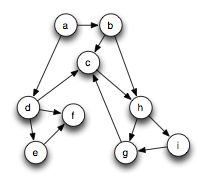
\includegraphics[width=0.5\textwidth]{aux/grafo}
		\caption[Estructura de un Grafo]{
		(tomada de \cite{BoostGrafos)}
		%\label{F-dimensions-emotion}
	\end{figure}


	\begin{figure}[H]
		\centering
		\includegraphics[width=0.5\textwidth]{aux/distributed_graph}
		\caption[Grafo Distribuido]{
		(tomada de \cite{BoostGrafos)}
		%\label{F-dimensions-emotion}
	\end{figure}
	
	

	\begin{figure}[H]
		\centering
		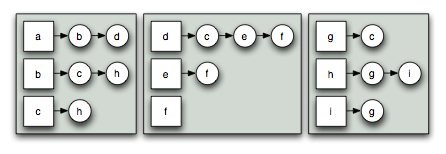
\includegraphics[width=0.5\textwidth]{aux/dist-adjlist}
		\caption[Grafo en lista de adyacencia]{
		(tomada de \cite{BoostGrafos)}
		%\label{F-dimensions-emotion}
	\end{figure}


	\begin{figure}[H]
		\centering
		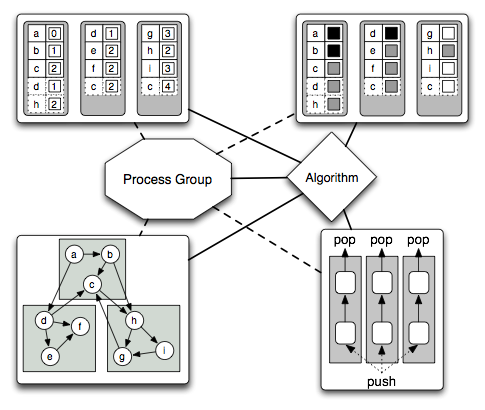
\includegraphics[width=0.5\textwidth]{aux/arquitectura_grafos}
		\caption[Aquitectura de Grafos]{
		(tomada de \cite{BoostGrafos)}
		%\label{F-dimensions-emotion}
	\end{figure}
	

	\section{C++}

	\section{MPI}

	\section{Boost}

	


	\section{Parallel Boost Graph Library}

	\begin{quotation}
		The Parallel Boost Graph Library is an extension to the Boost Graph Library (BGL) for parallel and distributed computing. It offers distributed graphs and graph algorithms to exploit coarse-grained parallelism along with parallel algorithms that exploit fine-grained parallelism, while retaining the same interfaces as the (sequential) BGL. Code written using the sequential BGL should be easy to parallelize with the parallel BGL. Visitors new to the Parallel BGL should read our architectural overview.\cite{wwwBoost} 
		\end{quotation} 

	\todo[inline,caption={TODO}]{Representacional}
